% Slides for 2025-04-22

\begin{frame}{Data Aug}
    \begin{itemize}
        \item Huggingface Datasets
        \item Experiments
        \item Collaboration with Sean on EGCI
    \end{itemize}
\end{frame}

\begin{frame}{EGCI}
    \centering
    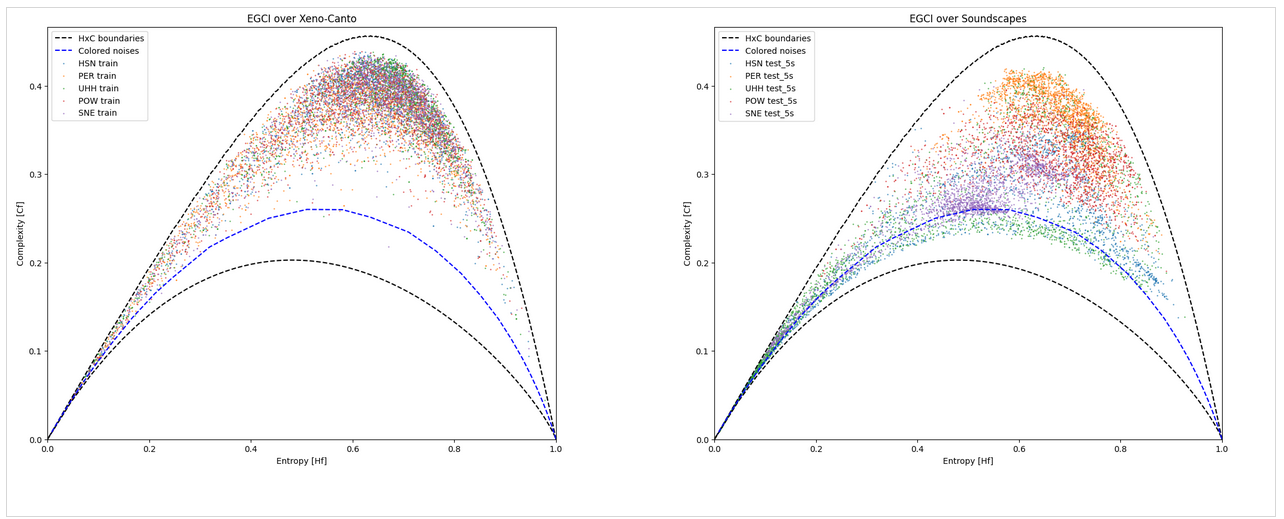
\includegraphics[height=0.7\textheight,width=0.7\textwidth,keepaspectratio]{images/EGCI_Example.png}
\end{frame}
\begin{frame}{Main Idea}
    can it describe the domain shift?
\end{frame}
\begin{frame}{How to Think About EGCI}
    \centering
    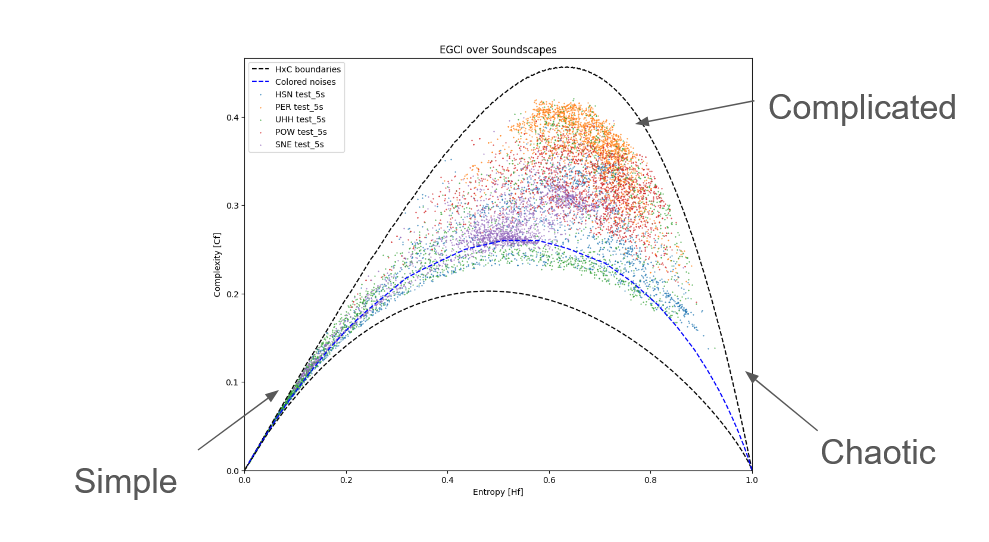
\includegraphics[height=0.7\textheight,width=0.7\textwidth,keepaspectratio]{images/intuition.png}
\end{frame}
\begin{frame}{Xeno-canto and Soundscapes}
    Experiment: EGCI features predict if a focal recording or a soundscape recording
    \centering
    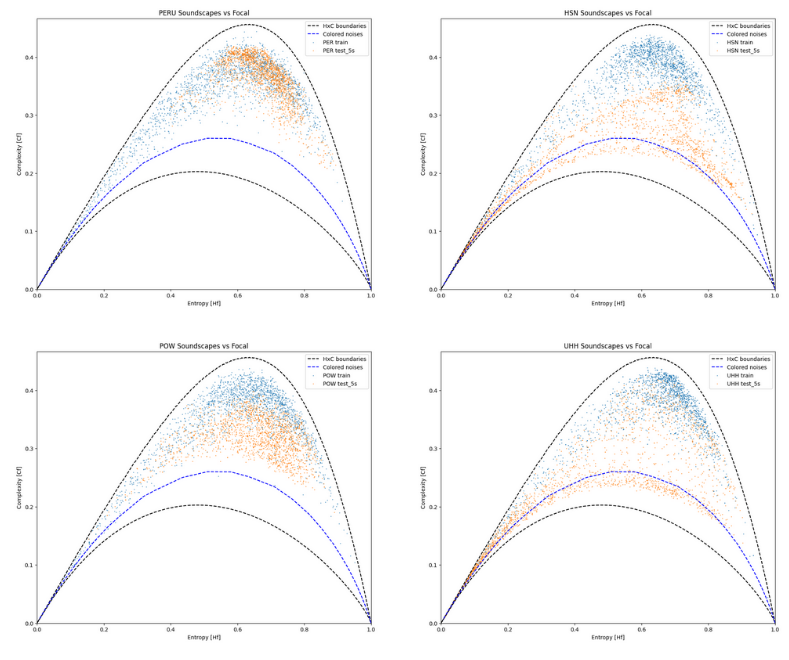
\includegraphics[height=0.9\textheight,width=0.9\textwidth,keepaspectratio]{images/region_compare.png} 
\end{frame}
\begin{frame}{Experiment Design}
    \begin{itemize}
        \item For each region
        \item train test split of focal and Soundscapes
        \item train svm, report test accuracy
        \item for significance, compare model accuracy to randomly assigning labels
        \item NULL: EGCI does not meaningfully represent the diff between focal and Soundscapes, thus isn't a useful feature
    \end{itemize}    
\end{frame}
\begin{frame}{Results}
    \begin{table}[]
        \begin{tabular}{l|ll}
        Region & Accuracy & p-value \\ \hline
        HSN    & 0.97625  & 0.0     \\
        PER    & 0.99875  & 0.0     \\
        UHH    & 0.96     & 0.0     \\
        POW    & 0.99375  & 0.0    
        \end{tabular}
    \end{table}  
\end{frame}
\begin{frame}{Results}
    \centering
    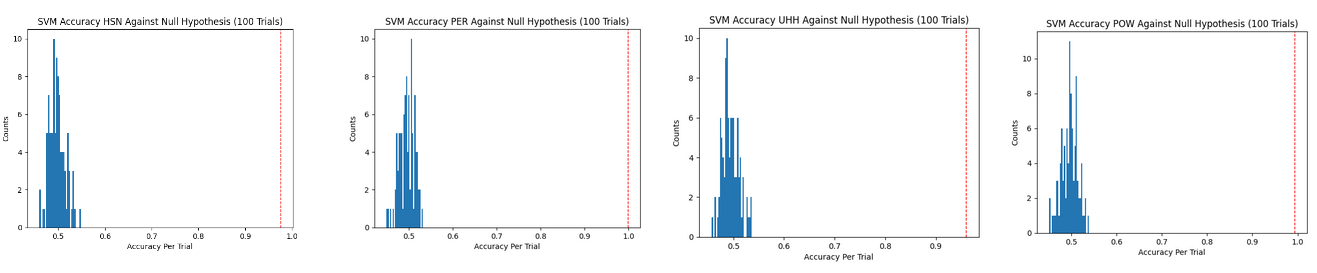
\includegraphics[height=2\textheight,width=1\textwidth,keepaspectratio]{images/Results.png} 
\end{frame}
\begin{frame}{Aside: On the Subject Matter of PER}
        \centering
        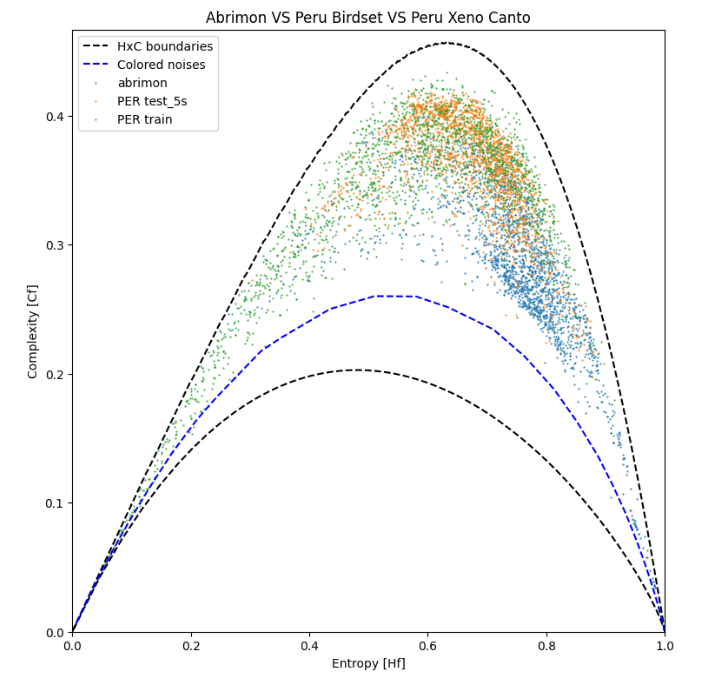
\includegraphics[height=0.7\textheight,width=0.7\textwidth,keepaspectratio]{images/AbrimonToo.png}  
\end{frame}
\begin{frame}{What does this ultimately mean for us?}   
    \centering
    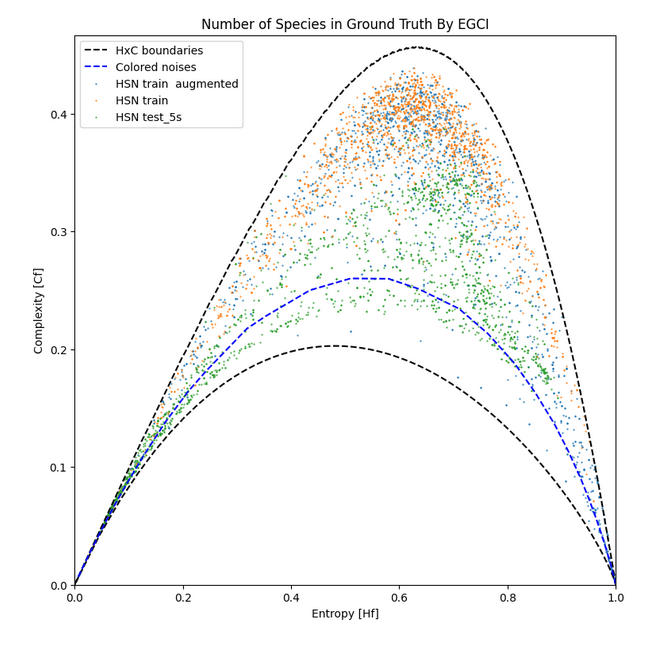
\includegraphics[height=0.7\textheight,width=0.7\textwidth,keepaspectratio]{images/dataAugExample.png}  
    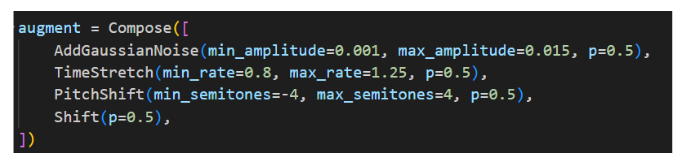
\includegraphics[height=0.7\textheight,width=0.7\textwidth,keepaspectratio]{images/augmentation.png}  
\end{frame}

























% To create a slide, use the following:
% \begin{frame}{TITLE}
%     BODY
% \end{frame}

% To create a slide with a bullet list, use the following:
% \begin{frame}{TITLE}
%     \begin{itemize}
%         \item ITEM 1
%         \item ITEM 2
%     \end{itemize}    
% \end{frame}

% To create a slide with numbered list, use the following:
% \begin{frame}{TITLE}
%     \begin{enumerate}
%         \item ITEM 1
%         \item ITEM 2
%     \end{enumerate}
% \end{frame}

% To create a slide with a graphic:
% 1. Add the graphic to this folder (named picture.png)
% 2. Use the following:
% \begin{frame}{TITLE}
%     \centering
%     \includegraphics[height=0.7\textheight,width=0.7\textwidth,keepaspectratio]{picture.png}
% \end{frame}

% To create a slide with two columns, use the following:
% \begin{frame}{TITLE}
%     \begin{columns}
%         \begin{column}{0.5\textwidth}
%             COLUMN 1 BODY
%         \end{column}
%         \begin{column}{0.5\textwidth}
%             COLUMN 2 BODY
%         \end{column}
%     \end{columns}
% \end{frame}
